\documentclass[12pt,hyperref,a4paper,UTF8]{ctexart}
\usepackage{HDUReport}
\usepackage{listings}
\usepackage{xcolor}
\usepackage{graphicx}
\usepackage{setspace}
\usepackage{float}
\setstretch{1.5} % 设置全局行距为1.5倍

\usepackage{enumitem} % 载入enumitem包以便自定义列表环境
\setlist[itemize]{itemsep=0pt, parsep=0pt} % 设置itemize环境的项目间距和段落间距

\setmainfont{Times New Roman} % 英文正文为Times New Roman


\usepackage{tikz}
\usetikzlibrary{shapes.geometric, arrows}
\usetikzlibrary{positioning, arrows.meta}
\usetikzlibrary{calc}
%封面页设置
{   
    %标题
    \title{ 
        \vspace{1cm}
        \heiti \Huge \textbf{《电磁波与电磁场实验》作业报告} \par
        \vspace{1cm} 
        \heiti \Large {\underline{实验5：微带缝隙天线的设计}   }     
    }

    \author{
        \kaishu\Large 指导教师\ \dlmu[9cm]{吴爱婷}  \\
        \kaishu\Large 学生姓名\ \dlmu[9cm]{陈文轩} \\ %学院
        \kaishu\Large 学生学号\ \dlmu[9cm]{23040447} \\ %
        \kaishu\Large 学生班级\ \dlmu[9cm]{23186011} \\ %班级
        \kaishu\Large 学生专业\ \dlmu[9cm]{智能硬件与系统(电子信息工程)} \qquad  \\ %学号
        \kaishu\Large 实验日期\ \dlmu[9cm]{2025.10.20} \qquad \\
         %姓名 
    }
        
    \date{\today} % 默认为今天的日期，可以注释掉不显示日期
}
%%------------------------document环境开始------------------------%%
\begin{document}

%%-----------------------封面--------------------%%
\cover
\thispagestyle{empty} % 首页不显示页码
%%------------------摘要-------------%%
%\newpage
%\begin{abstract}




%\end{abstract}

%\thispagestyle{empty} % 首页不显示页码

%%--------------------------目录页------------------------%%
% \newpage
% \tableofcontents
% \thispagestyle{empty} % 目录不显示页码

%%------------------------正文页从这里开始-------------------%
\newpage
\setcounter{page}{1} % 让页码从正文开始编号

%%可选择这里也放一个标题
%\begin{center}
%    \title{ \Huge \textbf{{标题}}}
%\end{center}

\section{实验目的}

1.通过此次实验，我们了解微带缝隙天线的概念

2.掌握 MWO EM structure 仿真方法

3.阻抗匹配掌握天线基本参数


\section{实验内容}


微带缝隙天线的仿真：

1.加载匹配结构的微带缝隙天线仿真

2.对于匹配结构的S11，3.75GHz点的db值应当尽量小；并在Smith图上，3.76GHz点尽量靠近图中心。

\subsection{主要实验步骤}

\textbf{1.新建工程，创建 EM structure，选择仿真器}

\begin{figure}[H]
  \centering
  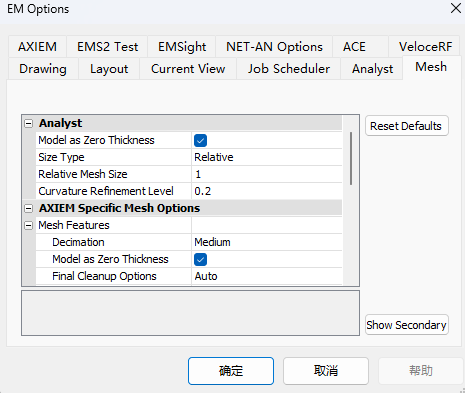
\includegraphics[width=0.8\textwidth]{figures/Emsight.png}
  \caption{Emsight设置界面}
  \label{fig:example}
\end{figure}

\textbf{2.设定 Enclosure，定义材料属性和边界条件}

\begin{figure}[H]
  \centering
  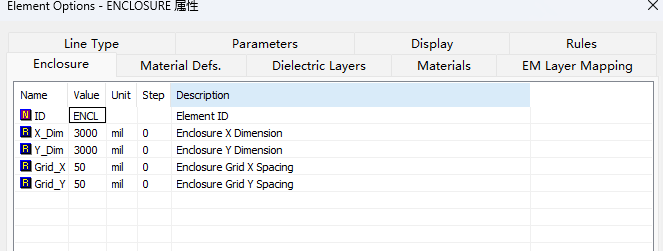
\includegraphics[width=1\textwidth]{figures/边界条件.png}
  \caption{Enclosure边界条件与材料层设置}
  \label{fig:enclosure}
\end{figure}

在AWR MWO的电磁仿真中，Enclosure（围盒）的设置至关重要，主要包括以下三个方面的配置：

(1) EM Layer Mapping（电磁层映射）

该界面用于将绘图层映射到电磁仿真层，实现物理结构到仿真模型的转换：

\begin{itemize}
    \item \textbf{Thick Metal层}：映射到EM Layer 2，对应实际的金属导体层（如微带线、天线辐射贴片等），该层具有一定厚度，在仿真中作为信号传输和辐射的主要结构；
    \item \textbf{Via Extent}：设置为Material 1，用于定义通孔（via）在介质层中的延伸范围；
    \item 其他绘图层（Error、Mesa、Gate等）均设置为[None]，表示这些层在当前仿真中不参与电磁计算；
    \item Active EM Mapping选择"Default"，LPF Name设置为"+EMSight1"，确保使用正确的仿真引擎。
\end{itemize}

(2) Dielectric Layers（介质层定义）

定义了三层介质结构的堆叠关系：

\begin{itemize}
    \item \textbf{Layer 1}：厚度300 mil，材料为Diel\_1（$\varepsilon_r = 1$，即空气层），作为天线上方的辐射空间；
    \item \textbf{Layer 2}：厚度30 mil，材料为Diel\_2（$\varepsilon_r = 2.33$，介质基板），这是微带线和天线结构的承载基板；
    \item \textbf{Layer 3}：厚度300 mil，材料为Diel\_1（$\varepsilon_r = 1$，空气层），作为天线下方的辐射空间。
\end{itemize}

这种"空气-基板-空气"的三明治结构模拟了微带缝隙天线在自由空间中的辐射环境。

(3) Material Defs（材料定义）

定义了两种介质材料的电磁参数：

\begin{itemize}
    \item \textbf{Diel\_1}：相对介电常数$\varepsilon_r = 1$，损耗角正切$\tan\delta = 0$，代表理想空气介质；
    \item \textbf{Diel\_2}：相对介电常数$\varepsilon_r = 2.33$，损耗角正切$\tan\delta = 1.3\times10^{-3}$，代表低损耗微波基板材料（如Rogers板材）。
\end{itemize}

材料的介电常数和损耗角正切直接影响微带线的特性阻抗、相位速度以及天线的辐射效率和带宽特性。通过Advanced Properties可以进一步设置材料的高级电磁参数（如各向异性、色散特性等）。


\textbf{3.创建辐射单元，添加端口，设定扫描频率}

在EM Structure中绘制微带缝隙天线的辐射单元，包括缝隙结构和馈电微带线。在馈电端添加端口（Port），并设定工作频率范围（1-8GHz），以便仿真天线在目标频段的电磁特性。

\begin{figure}[H]
  \centering
  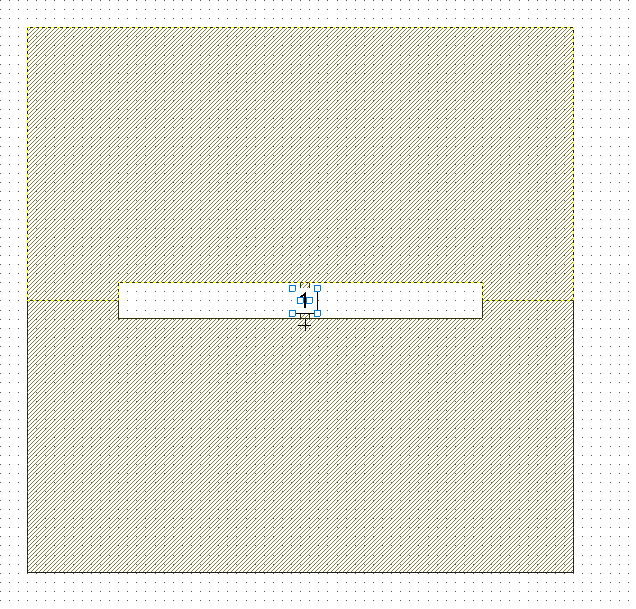
\includegraphics[width=0.9\textwidth]{figures/4.png}
  \caption{辐射单元结构与端口设置}
  \label{fig:radiation_element}
\end{figure}

\begin{figure}[H]
  \centering
  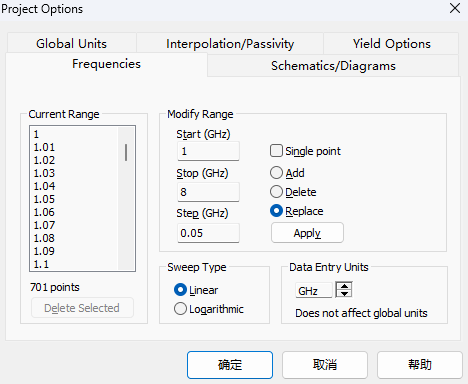
\includegraphics[width=0.9\textwidth]{figures/5.png}
  \caption{仿真范围与步长设置}
  \label{fig:radiation_element}
\end{figure}

\textbf{4.新增图表，增加测试量(S11、史密斯图)}

在MWO中新建测量图表，添加关键测试参量以评估天线性能：

\begin{itemize}
    \item \textbf{S11参数}：反射系数，用于评估天线在工作频段的输入匹配特性。
    \item \textbf{Smith圆图}：直观显示天线输入阻抗随频率的变化轨迹，便于进行阻抗匹配设计；在3.75GHz时，Smith线非常靠近图像中心，即此时阻抗匹配良好。
\end{itemize}

\begin{figure}[H]
  \centering
  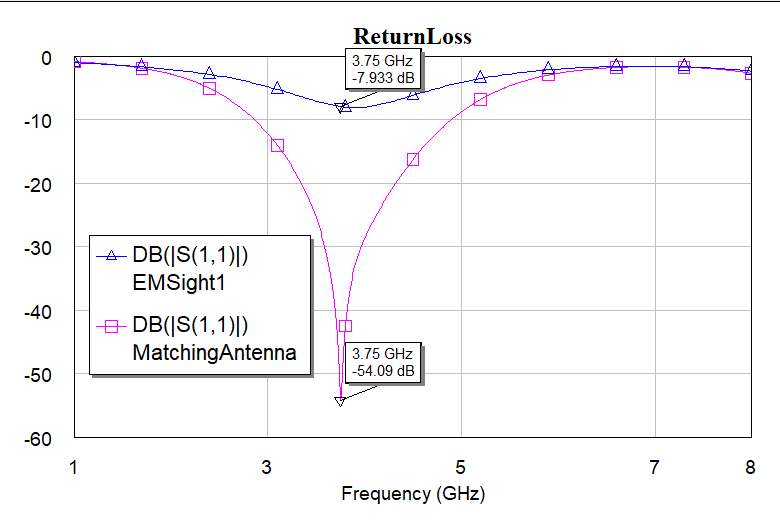
\includegraphics[width=0.9\textwidth]{figures/7.png}
  \caption{S11参数测量结果}
  \label{fig:s11_measurement}
\end{figure}

\begin{figure}[H]
  \centering
  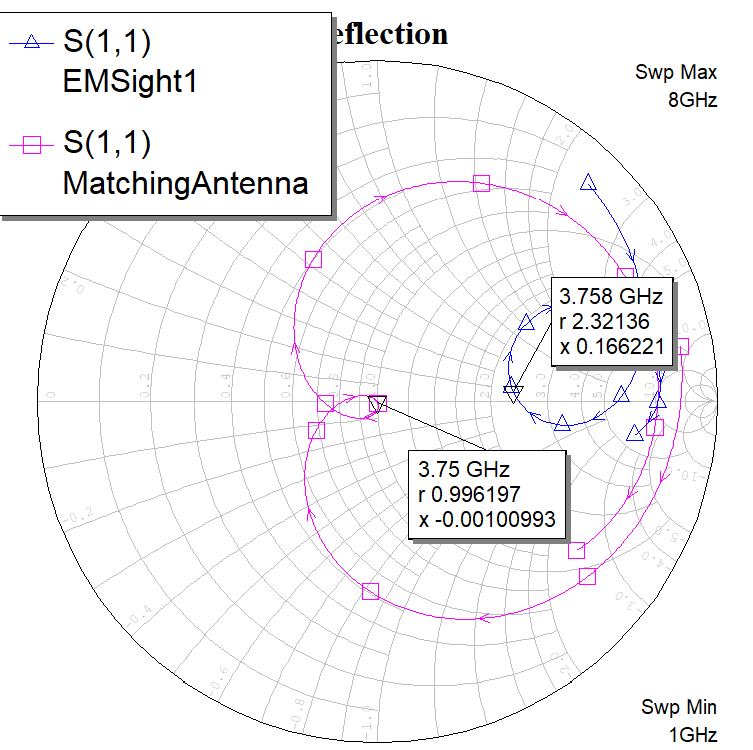
\includegraphics[width=0.9\textwidth]{figures/6.png}
  \caption{Smith圆图显示阻抗特性}
  \label{fig:smith_chart}
\end{figure}

\textbf{5.增加阻抗匹配微带线，搭建原理图，调节阻抗匹配}

由于天线输入阻抗通常不是标准的50$\Omega$，需要设计阻抗匹配网络。使用调谐工具调试不同特性阻抗的微带线宽度，在原理图中搭建匹配电路（如四分之一波长阻抗变换器或多段阻抗变换），通过优化调节各段微带线的长度和宽度参数，使3.75 GHz附近的S11值最小，Smith圆图上的轨迹尽量接近中心点（50$\Omega$匹配点）。

\begin{figure}[H]
  \centering
  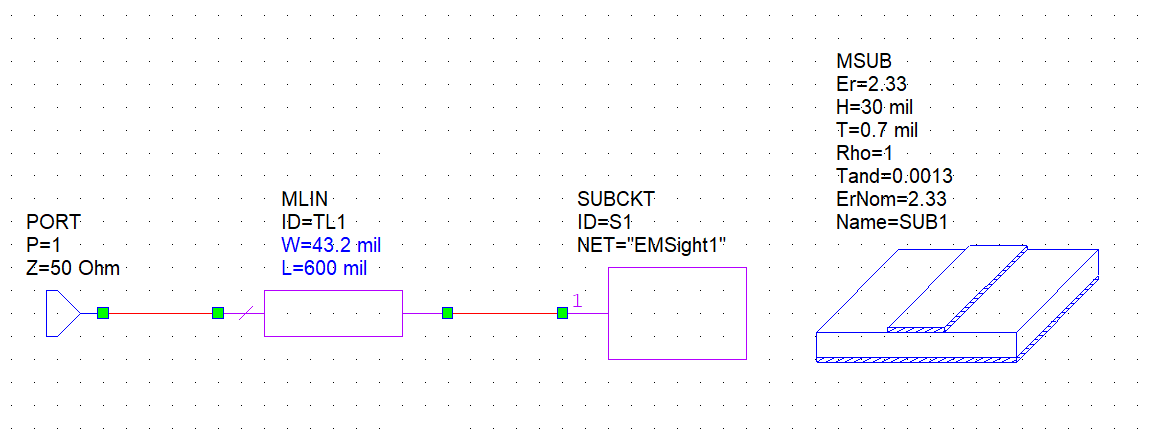
\includegraphics[width=0.9\textwidth]{figures/8.png}
  \caption{阻抗匹配网络原理图}
  \label{fig:matching_circuit}
\end{figure}



\textbf{6.观察辐射单元表面电流密度和缝隙辐射强度}

仿真完成后，通过EM Sight的后处理功能查看天线表面的电流分布和缝隙处的场强分布。电流密度图可以直观显示能量在天线结构上的分布情况，缝隙处的强电场表明该处为主要的辐射源，验证了微带缝隙天线的工作机理。

\begin{figure}[H]
  \centering
  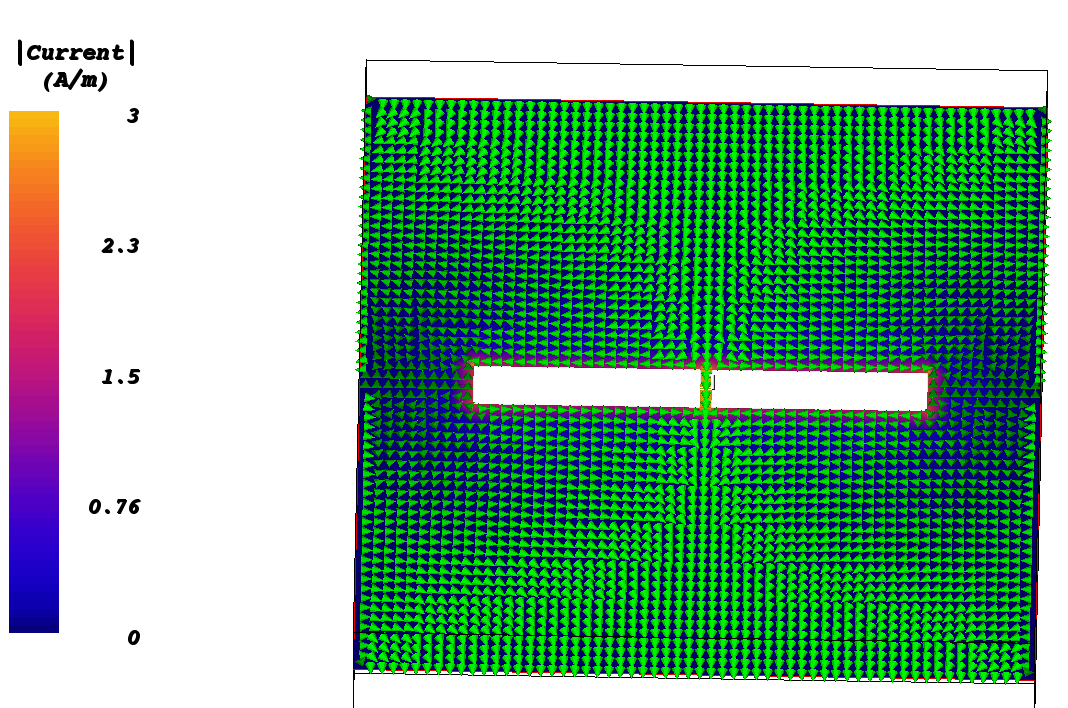
\includegraphics[width=0.9\textwidth]{figures/9.png}
  \caption{天线表面电流密度分布}
  \label{fig:current_density}
\end{figure}

\begin{figure}[H]
  \centering
  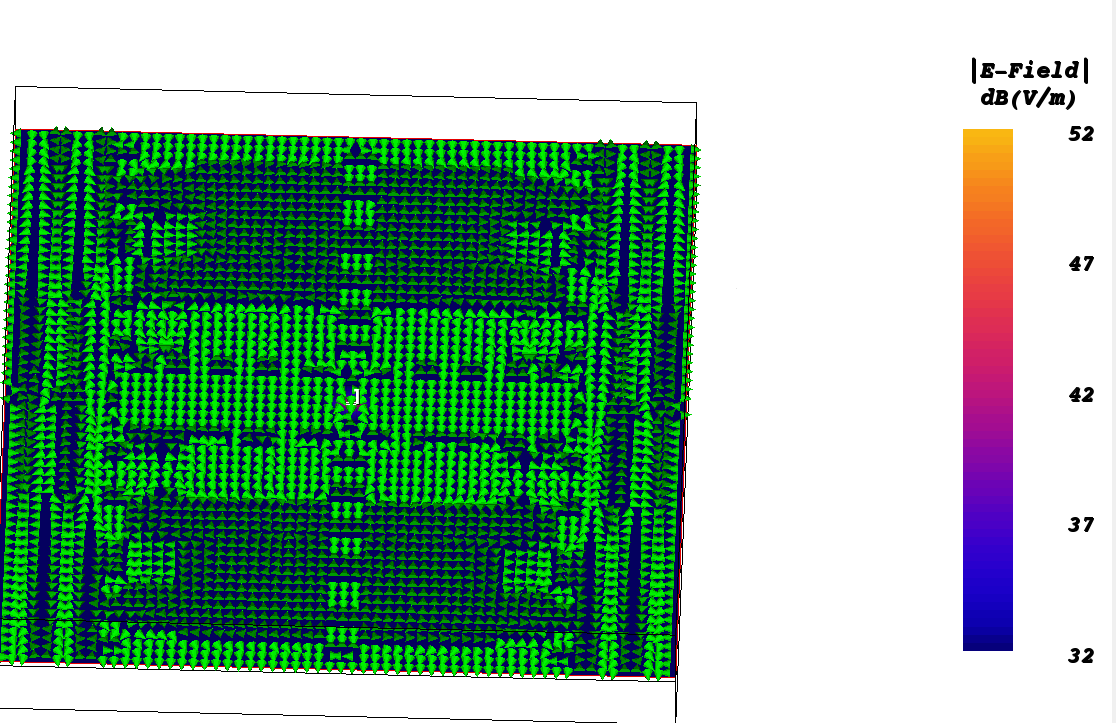
\includegraphics[width=0.9\textwidth]{figures/10.png}
  \caption{缝隙处的电场强度分布}
  \label{fig:field_distribution}
\end{figure}





\section{总结}

本次实验成功完成了微带缝隙天线的设计、仿真与阻抗匹配优化。通过使用AWR软件的EM Structure模块，初步进行了微带缝隙天线的设计。

在实验过程中，首先建立了"空气-基板-空气"的三层介质结构模型，其中介质基板采用相对介电常数$\varepsilon_r = 2.33$的低损耗材料。微带线的特性阻抗$Z_0$与基板参数的关系为：

$$Z_0 = \frac{60}{\sqrt{\varepsilon_{eff}}}\ln\left(\frac{8h}{W}+\frac{W}{4h}\right)$$

其中$\varepsilon_{eff}$为有效介电常数，$h$为基板厚度，$W$为微带线宽度。通过调整微带线几何尺寸，实现了50$\Omega$标准阻抗的匹配设计。

仿真结果表明，在目标频率3.75 GHz处，通过阻抗匹配网络的优化，S11参数达到最小值，Smith圆图上的轨迹接近中心点，证明天线实现了良好的阻抗匹配。电流密度和电场分布图直观展示了缝隙处为主要辐射源，验证了微带缝隙天线通过缝隙耦合辐射电磁波的工作机理。

通过本次实验，掌握了电磁仿真软件的基本操作流程，包括材料定义、边界条件设置、端口配置和结果分析等关键步骤，同时初步理解了天线阻抗匹配的重要性。

\end{document}